\chapter{Introducción}
\drop{A}{ctualmente} existen numerosos avances en lo que a las <<nuevas tecnologías>> se refiere y cada vez tenemos más dispositivos con los que comunicarnos y estar en contacto con amigos, familiares o conocidos en todo momento. De un tiempo a esta parte, hemos ido adoptando nuevas formas de comunicación en lo que respecta a los colegios, institutos, etc. Por ejemplo, antes se recurría al reparto de una circular para anunciar ciertos eventos a los alumnos para que se la entregaran a los padres o tutores. También se podía recurrir a escribir una nota en la agenda del alumno para que la entregase firmada al día siguiente si no había hecho los deberes asignados o había ocurrido algún percance. Posteriormente, se podría usar el correo electrónico para comunicarse directamente con los padres, asegurándose de la correcta recepción del comunicado, aunque pudiera ocurrir que éstos no lo revisaran en tiempo y forma. Hoy en día se dispone de los llamados \textit{smartphones} y la mensajería instantánea, con lo que los profesores pueden comunicarse en tiempo real con los padres y éstos pueden aportar algún tipo de \textit{feedback} en un corto periodo de tiempo.

Existen multitud de aplicaciones <<generalistas>> de mensajería instantánea que se describirán con detalle en un capítulo posterior (\ref{chap:antecedentes}: \nameref{chap:antecedentes}). No obstante, la comunidad autónoma de Castilla-La Mancha posee la plataforma educativa llamada <<Papás 2.0>>.

\section*{Papás 2.0}

Papás 2.0 (figura \ref{fig:papas20}) se encuentra más enfocada al sector docente, al igual que la aplicación que se pretende desarrollar. Se trata de una plataforma educativa perteneciente a la Consejería de Educación, Cultura y Deportes de la \acf{JCCM}. Facilita la gestión administrativa y establece una vía de comunicación entre los centros educativos y las familias, ofreciendo información en tiempo real \cite{JCCM2017}. Además, permite llevar un seguimiento sobre las tareas, trabajos, controles, exámenes, faltas de asistencia y fechas de entrega \cite{JCCM2010}.

\begin{figure}[!h]
	\begin{center}
		
\includegraphics[width=0.4\textwidth]{/logo_papas_20}
		\caption{Logo de Papás 2.0}
		\label{fig:papas20}
	\end{center}
\end{figure}

\newpage

Papás 2.0 ofrece una serie de características principalmente enfocadas a los padres, siendo éstas las más destacadas \cite{JCCM2010}:

\begin{itemize}
	\item Visualizar los profesores que dan clase a los hijos con sus datos y posibilidad de escribir un mensaje directamente a cualquiera de ellos.
	\item Consultar las citas concertadas con los profesores, junto con la fecha, hora y motivo de la visita.
	\item Consultar el horario escolar.
	\item Consultar las faltas de asistencia, con la posibilidad de ser notificado vía SMS o correo electrónico. Del mismo modo, se podrá registrar una notificación cuando se sepa que el hijo va a faltar a ciertas horas.
	\item Consultar trabajos y tareas de cada hijo, así como ver las fechas de los exámenes y sus notas del curso y su trayectoria escolar.
	\item Envío y recepción de mensajes mediante grupos, como el de madres y padres, pudiendo adjuntar archivos de tamaño no superior a 1\acs{MB} y con un máximo de 3\acs{MB} en total.
\end{itemize}

\section*{Problemas comunes con las aplicaciones de mensajería}
Aunque existen diversas soluciones para la comunicación entre los padres y el centro en el que se encuentren sus hijos y aportan numerosos beneficios a la comunidad educativa, muchas veces se pueden producir malentendidos cuando se hace uso de la mensajería instantánea, entre otros problemas. Además, también se producen situaciones poco deseables entre los padres.

\newpage

\subsection*{Celebraciones desafortunadas}
En este caso, un grupo de madres se negaba a llevar a sus hijos al colegio debido a que a la clase de éstos acudía un niño que sufría síndrome de Asperger. Sucedió en Buenos Aires, Argentina, y pronto se dio a conocer en Internet.
En las capturas de la conversación (figura \ref{fig:whatasper}) se puede ver cómo las madres se alegran de que este chico fuera cambiado de clase. <<Una buenísima noticia>>, según indicaba una de las madres \cite{Vanguardia2017}.

\begin{figure}[!h]
	\begin{center}
		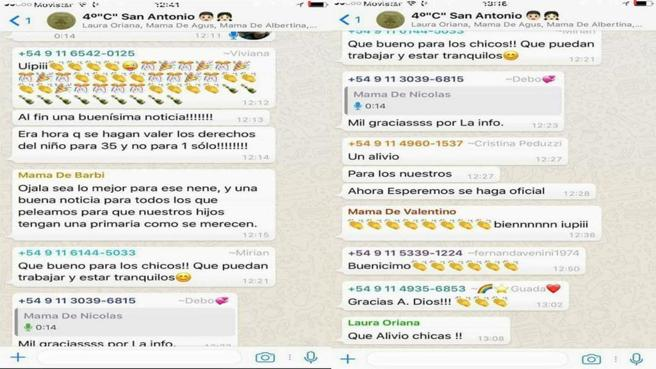
\includegraphics[width=0.8\textwidth]{/whatsapp_asperger}
		\caption{Captura conversación madres}
		\label{fig:whatasper}
	\end{center}
\end{figure}

\subsection*{Uso de los grupos para compartir deberes hechos}
Más allá de los problemas que puedan surgir entre los padres, los grupos pueden llegar incluso a dañar a los propios hijos. Esto puede suceder puesto que hay padres que comparten el trabajo realizado en casa para que otros niños o padres puedan beneficiarse de ello. Esta práctica puede repercutir en un mal aprendizaje del niño y, por tanto, en una disminución de su rendimiento escolar. Incluso pueden llegar a compartir fotos de los regalos colocados debajo del árbol en la época navideña \cite{Alias2017}. Por todo esto se debe establecer de manera firme y consensuada la figura del administrador del grupo, que será quien se encargue del cumplimiento y gestión de las normas para que la relación y saber estar de los padres no se quede sólo en el trato presencial sino que se extrapole a las nuevas soluciones digitales.

\subsection*{Grupos escolares para hablar de todo}
En este caso, una madre mandó una carta a la autora de la noticia. Sucedió en Argentina y en ella explica cómo, a raíz de abandonar el grupo de madres, éstas la tratan de una manera diferente. El motivo principal era que en dicho grupo se hablaba demasiado, llegando a ser <<insoportables>>, decía la madre. Lo que pensaba se confirmó al necesitar a una madre para que recogiera a su hija, asegurando que le devolvería el favor la próxima vez. Esta madre leyó e ignoró el mensaje y, posteriormente, alegó que no se había dado cuenta \cite{Consuelo2017}.

%\section{Título del proyecto}
%En la portada ---y otras páginas de presentación--- el nombre o título del
%proyecto debe aparecer sin comillas, cursiva u otros formatos. Si se cita el
%título de otra obra, o el nombre de un capítulo sí debe aparecer entre
%comillas. Por cierto, las comillas que deben usarse en castellano son las
%«latinas», dejando las ``inglesas'' para los raros casos en los que aparezca una
%cita en el cuerpo otra~\cite{sousa}.
%
%\section{Estructura del documento}
%Pueden incluirse aquí una sección con algunos consejos para la lectura del
%documento dependiendo de la motivación o conocimientos del lector.  También
%puede ser útil incluir una lista con el nombre y finalidad de cada uno de los
%capítulos restantes.
%
%\begin{definitionlist}
%\item[Capítulo \ref{chap:antecedentes}: \nameref{chap:antecedentes}] Explica herramientas
%  y aspectos básicos de edición con \LaTeX.
%\item[Capítulo \ref{chap:objetivos}: \nameref{chap:objetivos}] Finalidad y justificación
%  (con todo detalle) del presente documento.
%\end{definitionlist}

% Local Variables:
%  coding: utf-8
%  mode: latex
%  mode: flyspell
%  ispell-local-dictionary: "castellano8"
% End: